% me=0 student solutions (ps file), me=1 - my solutions (sol file),
% me=2 - assignment (hw file)
\def\me{0} \def\num{4} %homework number

\def\due{11:55 pm on Thursday, March 7} %due date

\def\course{CSCI-UA 310-007, Basic Algorithms} %course name, changed only once

% **** INSERT YOUR NAME HERE ****
\def\name{Yan Konichshev}

% **** INSERT YOUR NETID HERE ****
\def\netid{yk2602}

% **** INSERT NETIDs OF YOUR COLLABORATORS HERE ****
\def\collabs{N/A, N/A}


\iffalse

INSTRUCTIONS: replace # by the homework number.  (if this is not
ps#.tex, use the right file name)

Clip out the ********* INSERT HERE ********* bits below and insert
appropriate LaTeX code.  There is a section below for student macros.
It is not recommended to change any other parts of the code.


\fi
%

\documentclass[11pt]{article}


% ==== Packages ====
\usepackage{amsfonts,amsmath}
\usepackage{tkz-graph}
\usepackage{latexsym}
\usepackage{etoolbox}
\usepackage{totcount}
\usepackage{fullpage}
\usepackage{graphicx}
\usepackage{tikz}
\usepackage{tikz-qtree}
\usepackage[bottom]{footmisc}
\usepackage{enumitem}
\usepackage{hyperref}
\usepackage{mathtools}
\usepackage{graphicx}
\usepackage{listings}
\DeclarePairedDelimiter\ceil{\lceil}{\rceil}
\DeclarePairedDelimiter\floor{\lfloor}{\rfloor}

\setlength{\footskip}{1in} \setlength{\textheight}{8.5in}

\newcommand{\handout}[5]{
	\renewcommand{\thepage}{#1, Page \arabic{page}}
	\noindent
	\begin{center}
		\framebox{ \vbox{ \hbox to 5.78in { {\bf \course} \hfill #2 }
				\vspace{4mm} \hbox to 5.78in { {\Large \hfill #5 \hfill} }
				\vspace{2mm} \hbox to 5.78in { {\it #3 \hfill #4} }
				\ifnum\me=0
				\vspace{2mm} \hbox to 5.78in { {\it Collaborators: \collabs
						\hfill} }
				\fi
		} }
	\end{center}
	\vspace*{4mm}
}

\newcounter{pppp}
\newcounter{pppc}
\newcommand{\prob}{\arabic{pppp}} %problem number
\newcommand{\increase}{\stepcounter{pppp}\stepcounter{pppc}} %problem number

% Arguments: Title, Number of Points
\newcommand{\newproblem}[2]{
	\increase
	\restartlist{subtasks}
	\ifnum\me=0
	\ifnum\prob>0 \newpage \fi
	\setcounter{page}{1}
	\handout{\name{} (\netid), Homework \num, Problem \arabic{pppp}}
	{\today}{Name: \name{} (\netid)}{Due: \due}
	{Solutions to Problem \prob\ of Homework \num\ (#2)}
	\else
	\section*{Problem \num-\prob~(#1) \hfill {#2}}
	\fi
}

\newlist{subtasks}{enumerate}{1}
\setlist[subtasks]{label={(\alph*)},resume}

\newcounter{numpppp}
\loop
\stepcounter{numpppp}
% workaround bug in totcount (means \newtotcounter{points\arabic{pointsct}})
\begingroup%
\edef\tempcounter@@name{points\arabic{numpppp}}%
\expandafter\newtotcounter\expandafter{\tempcounter@@name}%
\edef\tempcounter@@name{ecpoints\arabic{numpppp}}%
\expandafter\newtotcounter\expandafter{\tempcounter@@name}%
\endgroup
\ifnum \value{numpppp}<500 % max number of tasks supported
\repeat

% formating of output
\newcommand{\disppoints}[1]{%
	\texorpdfstring{(#1~\ifnumequal{#1}{1}{point}{points})}{}
}

% adds and displays
\newcommand{\points}[1]{%
	\texorpdfstring{\addtocounter{points\arabic{pppc}}{#1}\disppoints{#1}}{}%
}
\newcommand{\ecpoints}[1]{%
	\texorpdfstring{\addtocounter{ecpoints\arabic{pppc}}{#1}\ec \disppoints{#1}}{}%
}

% total points of current task         
\newcommand{\currentpoints}{% total points of current task   
	\texorpdfstring{\ifnumequal{\totvalue{ecpoints\arabic{pppc}}}{0}%
		{\total{points\arabic{pppc}} points}%
		{\total{points\arabic{pppc}}+\total{ecpoints\arabic{pppc}} points}}{}%
}

\newcommand{\mixedpoints}[2]{%
	\texorpdfstring{%
		\addtocounter{points\arabic{pppc}}{#1}%
		\addtocounter{ecpoints\arabic{pppc}}{#2}%
		(#1 (+#2) points)
	}{}%
}


\def\squarebox#1{\hbox to #1{\hfill\vbox to #1{\vfill}}}
\def\qed{\hspace*{\fill}
	\vbox{\hrule\hbox{\vrule\squarebox{.667em}\vrule}\hrule}}
\newenvironment{solution}{\begin{trivlist}\item[]{\bf Solution:}}
	{\qed \end{trivlist}}
\newenvironment{solsketch}{\begin{trivlist}\item[]{\bf Solution
			Sketch:}} {\qed \end{trivlist}}
\newenvironment{code}{\begin{tabbing}
		12345\=12345\=12345\=12345\=12345\=12345\=12345\=12345\= \kill }
	{\end{tabbing}}


\newcommand{\hint}[1]{({\bf Hint}: {#1})}
% Put more macros here, as needed.
\newcommand{\room}{\medskip\ni}
\newcommand{\brak}[1]{\langle #1 \rangle}
\newcommand{\bit}[1]{\{0,1\}^{#1}}
\newcommand{\zo}{\{0,1\}}
\newcommand{\C}{{\cal C}}

\newcommand{\nin}{\not\in}
\newcommand{\set}[1]{\{#1\}}
\renewcommand{\ni}{\noindent}
\renewcommand{\gets}{\leftarrow}
\renewcommand{\to}{\rightarrow}
\newcommand{\assign}{:=}

\newcommand{\AND}{\wedge}
\newcommand{\OR}{\vee}
\newcommand{\For}{\mbox{\bf for }}
\newcommand{\To}{\mbox{\bf to }}
\newcommand{\DownTo}{\mbox{\bf downto }}
\newcommand{\Do}{\mbox{\bf do }}
\newcommand{\If}{\mbox{\bf if }}
\newcommand{\Then}{\mbox{\bf then }}
\newcommand{\Else}{\mbox{\bf else }}
\newcommand{\Elif}{\mbox{\bf elif }}
\newcommand{\While}{\mbox{\bf while }}
\newcommand{\Repeat}{\mbox{\bf repeat }}
\newcommand{\Until}{\mbox{\bf until }}
\newcommand{\Return}{\mbox{\bf return }}
\newcommand{\Halt}{\mbox{\bf halt }}
\newcommand{\Swap}{\mbox{\bf swap }}
\newcommand{\Ex}[2]{\textrm{exchange } #1 \textrm{ with } #2}
\newcommand{\Nil}{\mbox{\bf nil}}
\newcommand{\In}{\mathsf{inOrder}}
\newcommand{\Post}{\mathsf{postOrder}}
\newcommand{\Pre}{\mathsf{preOrder}}
\newcommand{\Root}{\mathsf{root}}
\newcommand{\Parent}{\mathsf{parent}}
\newcommand{\Left}{\mathsf{left}}
\newcommand{\Right}{\mathsf{right}}
\newcommand{\Middle}{\mathsf{middle}}
\newcommand{\True}{\textbf{true}}
\newcommand{\False}{\textbf{false}}
\newcommand{\Print}{\mbox{\bf print }}
\newcommand{\ec}{({\bf Extra Credit})}
\newcommand{\note}{{\bf Note to Graders: }}
\newcommand{\Rotate}{\textsc{Rotate}}
\newcommand{\LRotate}{\textsc{LeftRotate}}
\newcommand{\RRotate}{\textsc{RightRotate}}

\newcommand{\notename}[2]{{\textcolor{red}{\footnotesize{\bf (#1:} {#2}{\bf ) }}}}
\newcommand{\sparsh}[1]{{\notename{Sparsh}{#1}}}

\newcommand{\noname}[2]{{\textcolor{purple}{\footnotesize{\bf (#1:} {#2}{\bf ) }}}}
\newcommand{\tanmay}[1]{{\noname{Tanmay}{#1}}}
\newcommand{\Gray}{\textsc{gray}}
\newcommand{\White}{\textsc{white}}
\newcommand{\Black}{\textsc{black}}

\begin{document}

\ifnum\me=0

% Collaborators (on a per task basis):
%
% Task 1: *********** INSERT COLLABORATORS HERE *********** 
% Task 2: *********** INSERT COLLABORATORS HERE *********** 
% etc.  
%

\fi

% \handout{\name{} (\netid), Homework \num, Problem \arabic{pppp}}
% 	{\today}{Name: \name{} }{Due: \due}
% 	{Homework 4}

\newproblem{Collaborators}{0 points}
    \noindent
Add the names and NetID(s) of your collaborators at the start of your solution file. If you haven't collaborated with anyone then say none. Do not leave it blank! You are allowed to consult external resources but you must write the solutions on your own keeping your resources closed. You must mention your resources here. 
\ifnum\me<2
\begin{solution}\\
N/A  
\end{solution}
\fi

\newproblem{Overscrupulous}{\currentpoints}


\noindent



\begin{subtasks}

	\item \points{2} Draw an undirected graph for the following adjacency matrix.
\[
\begin{array}{c|cccccccc}
& 0 & 1 & 2 & 3 & 4 & 5 & 6 & 7 \\
\hline
0 & 0 & 0 & 1 & 0 & 0 & 0 & 0 & 0 \\
1 & 0 & 0 & 0 & 1 & 0 & 0 & 0 & 0 \\
2 & 1 & 0 & 0 & 1 & 1 & 0 & 0 & 1 \\
3 & 0 & 1 & 1 & 0 & 0 & 1 & 0 & 0 \\
4 & 0 & 0 & 1 & 0 & 0 & 0 & 0 & 1 \\
5 & 0 & 0 & 0 & 1 & 0 & 0 & 0 & 1 \\
6 & 0 & 0 & 0 & 0 & 0 & 0 & 0 & 1 \\
7 & 0 & 0 & 1 & 0 & 1 & 1 & 1 & 0 \\
\end{array}
\]
 \ifnum\me<2
\begin{solution}

\begin{tikzpicture}
\tikzset{vertex/.style = {shape=circle,draw,minimum size=1.5em}}
% vertices
\foreach \x/\name in {0/0,1/1,2/2,3/3,4/4,5/5,6/6,7/7} {
    \node[vertex] (\name) at (\x*360/8:4cm) {$\name$};
}
% edges
\foreach \i/\j in {0/2,1/3,2/0,2/3,2/4,2/7,3/1,3/2,3/5,4/2,4/7,5/3,5/7,6/7,7/2,7/4,7/5,7/6} {
    \draw (\i) -- (\j);
}
\end{tikzpicture}

\end{solution}
	\fi

 \item \points{2}
        Draw a directed graph for the following adjacency list.
        \begin{align*}
0 & \rightarrow [1, 5] \\
1 & \rightarrow [7] \\
2 & \rightarrow [7] \\
3 & \rightarrow [2, 4, 7] \\
4 & \rightarrow [2, 6] \\
5 & \rightarrow [3] \\
6 & \rightarrow [2, 3] \\
7 & \rightarrow [0] \\
\end{align*}

  \ifnum\me<2
\begin{solution}

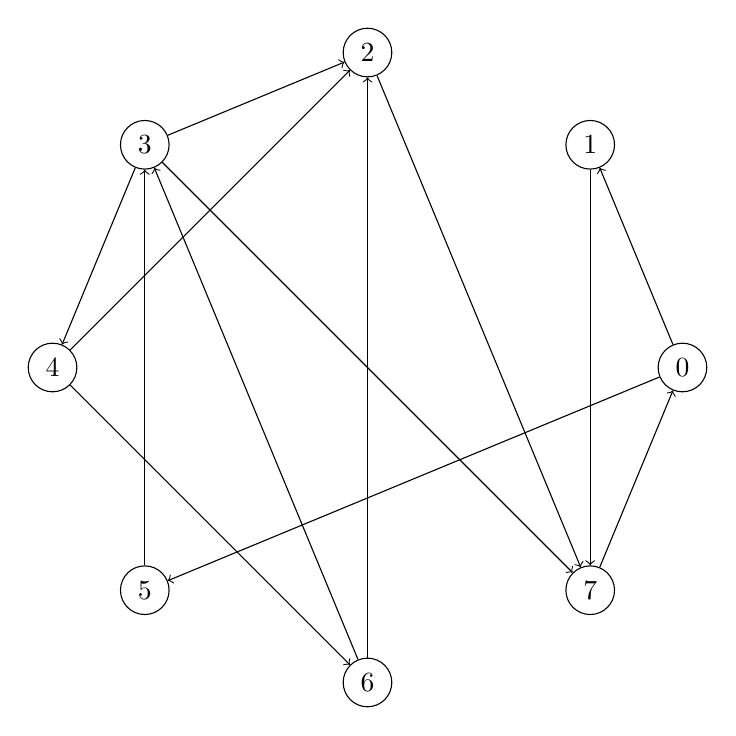
\begin{tikzpicture}
\tikzset{vertex/.style = {shape=circle,draw,minimum size=1.5em}}
% vertices
\foreach \x/\name in {0/0,1/1,2/2,3/3,4/4,5/5,6/6,7/7} {
    \node[vertex] (\name) at (\x*360/8:4cm) {$\name$};
}
% edges
\foreach \i/\j in {0/1,0/5,1/7,2/7,3/2,3/4,3/7,4/2,4/6,5/3,6/2,6/3,7/0} {
    \draw[->] (\i) -- (\j);
}
\end{tikzpicture}

\end{solution}
	\fi

  \item \points{4} 
Run both BFS and DFS on the graph from part (b) starting from node $0$. Show the BFS and DFS trees and classify the edges.     
  \ifnum\me<2
\begin{solution}\\

BFS: 0, 5, 1, 3, 7, 4, 2, 6\\
DFS: 0, 1, 7, 5, 3, 2, 4, 6\\
See the attachment for the trees and edge labels.

\end{solution}
	\fi


  \item \points{4} 
Modify the pseudocode for DFS so that it prints out every edge in the directed graph $G$ along with its type. 
  \ifnum\me<2
\begin{solution}\\

\begin{lstlisting}[language=Python, caption=depth-first search]

def modified_DFS(D):

    for i in range(len(n)):
        color[i] = white 
        parent[i] = -1
        
    time = 0
    for i in range(len(n)):
        if color[i] is white:
            DFS_Visit(i)
    
def DFS_Visit(i):

    time = time + 1
    start[i] = time
    color[i] = grey
    
    for neighbor in i.neighbors(): 
        
        
        if color[neighbor] == white: 
            # printing the tree edge 
            print("Tree-Edge:", neighbor, "->", i);
            parent[neighbor] = i
            modified_DFS(neighbor)

        if color[neighbor] == grey:
            # printing the back edge 
            print("Back-Edge:", neighbor, "->", i);
            return True
    
    time = time + 1
    finish[i] = count 
    color[i] = black
    
\end{lstlisting}

\end{solution}
	\fi

 \item \points{2} What is a minimal set of edges that needs to be removed from (b) to turn it into a Directed Acyclic Graph (DAG)?

  \ifnum\me<2
\begin{solution}   INSERT YOUR SOLUTION HERE   \end{solution}
	\fi

\end{subtasks}
 
\newproblem{Losing My Way}{\currentpoints}

You have just assumed the role of student welfare coordinator at Newest University of York. The University has several buildings on different streets on an island. You decide to do some investigative work, you model the buildings and the path between them as a graph (Note that for any two vertices, there can only be one undirected edge between them). Your network is represented as an \textbf{undirected} graph $G=(V,E)$ with $n$ buildings connected by $m$ edges. You have determined that the graph is indeed \textbf{connected}. With all the construction on campus, you realize that there are not enough redundant paths to ensure connectivity in case of a building being blocked. You have a limited budget so you decide that the best you can do is to avoid any single point of failure. A single point of failure is a building which when walled off disconnects the network into different components.

\begin{subtasks}

\item \points{2} 
Give a sample graph with $8$ nodes that contains EXACTLY \textbf{one} single point of failure.
 \ifnum\me<2
\begin{solution} \\

Please see the attachment below for the detailed picture of how this could be possible.

\end{solution}
	\fi

 \item \points{6}
You want to test if a given node $w$ is a single point of failure. You will do this by modifying
	the standard BFS algorithm.
	Suitably modify the algorithm to write the pseudocode
	for {\sc SPOF}$(G,s,w)$ that returns $\True$ if $w$
	is a single point of failure and \False\ otherwise. 
	Here $s\neq w$ is an arbitrary node from which you begin
	exploring. Briefly argue why your algorithm works and state the running time  of the algorithm.
	
	 \ifnum\me<2
\begin{solution}   INSERT YOUR SOLUTION HERE   \end{solution}
	\fi


 \item \ecpoints{6}
You are given a	node $u$ and are told that there exists
	a node $v$ such that $\delta(u,v)>n/2$. Here $\delta(u,v)$ denotes the 
	shortest distance (in the number of edges) between $u$ and $v$.
	This means that the two nodes are really far apart.
	You have an intuition that there
	might be a single point of failure that would
	disrupt the connection between $u$ and $v$ given
	the large distance between them. 
	Specifically, you fear that there is a distinct
	building $w$ which breaks
	all paths between servers $u$ and $v$ when it
	is walled off. 

	
	Give an algorithm running in time $O(m+n)$ to find the node $w$. Argue why your algorithm works and state the running time of your algorithm.

 \ifnum\me<2
\begin{solution}   INSERT YOUR SOLUTION HERE   \end{solution}
	\fi
 \end{subtasks}
Having finished your internship, you scurry over to your grumpy Algorithms Teaching Assistant. Instead of giving you extra credit for your wondrous work, he asks you to argue why the following assertions are correct to check if you really did the work you say you did.


\begin{subtasks}
    
  \item \points{6}
    \begin{itemize}
    \item The root of the DFS tree is a single point of failure if and only if it has two or more children.
    \item No leaf of the DFS tree can be a single point of failure.
    \item A non-root, internal vertex \(u\) of the DFS tree is a single point of failure if and only if it has a child \(v\) such that no back edge of \(v\)'s subtree goes to a proper ancestor of \(u\).
\end{itemize}
Hint : Utilize proof by contradiction and remember that $G$ is undirected.
 \ifnum\me<2
\begin{solution}   INSERT YOUR SOLUTION HERE   \end{solution}
	\fi

\end{subtasks}

\newproblem{Applicative Questions}{\currentpoints}

\begin{subtasks}

\item \points{4}
Given a list of \( n \) professional basketball players and a list of \( r \) pairs indicating rivalries between them, the objective is to determine if it is feasible to classify the players into two groups: shooters and dunkers. The classification should be done in such a way that each rivalry is between one shooter and one dunker. The algorithm should have a time complexity of \( O(n + r) \). If such a classification is possible, the algorithm should also specify the grouping.

\ifnum\me<2
\begin{solution}   INSERT YOUR SOLUTION HERE   \end{solution}
	\fi

 \item \points{2}
	Give a counterexample to the conjecture that if a directed graph \( G \) contains a path from \( u \) to \( v \), and if \( start[u] < start[v] \) in a depth-first search of \( G \), then \( v \) is a descendant of \( u \) in the depth-first forest produced. 
 

	\ifnum\me<2
\begin{solution}   INSERT YOUR SOLUTION HERE   \end{solution}
	\fi

 \item \points{2}
	Give a counterexample to the conjecture that if a directed graph \( G \) contains a path from \( u \) to \( v \), then any depth-first search must result in \(start[v]\leq finish[u] \).
 

	\ifnum\me<2
\begin{solution}   INSERT YOUR SOLUTION HERE   \end{solution}
	\fi


 \item \points{6}Given a directed graph $G = (V, E)$ where edges are either red or blue, find the shortest RB-path from $s$ to every other node $v \in V$. An RB-path is a path where the edges alternate colors between red and blue.

	\ifnum\me<2
\begin{solution}   INSERT YOUR SOLUTION HERE   \end{solution}
	\fi



    
\end{subtasks}
\end{document}


